\pagenumbering{gobble}

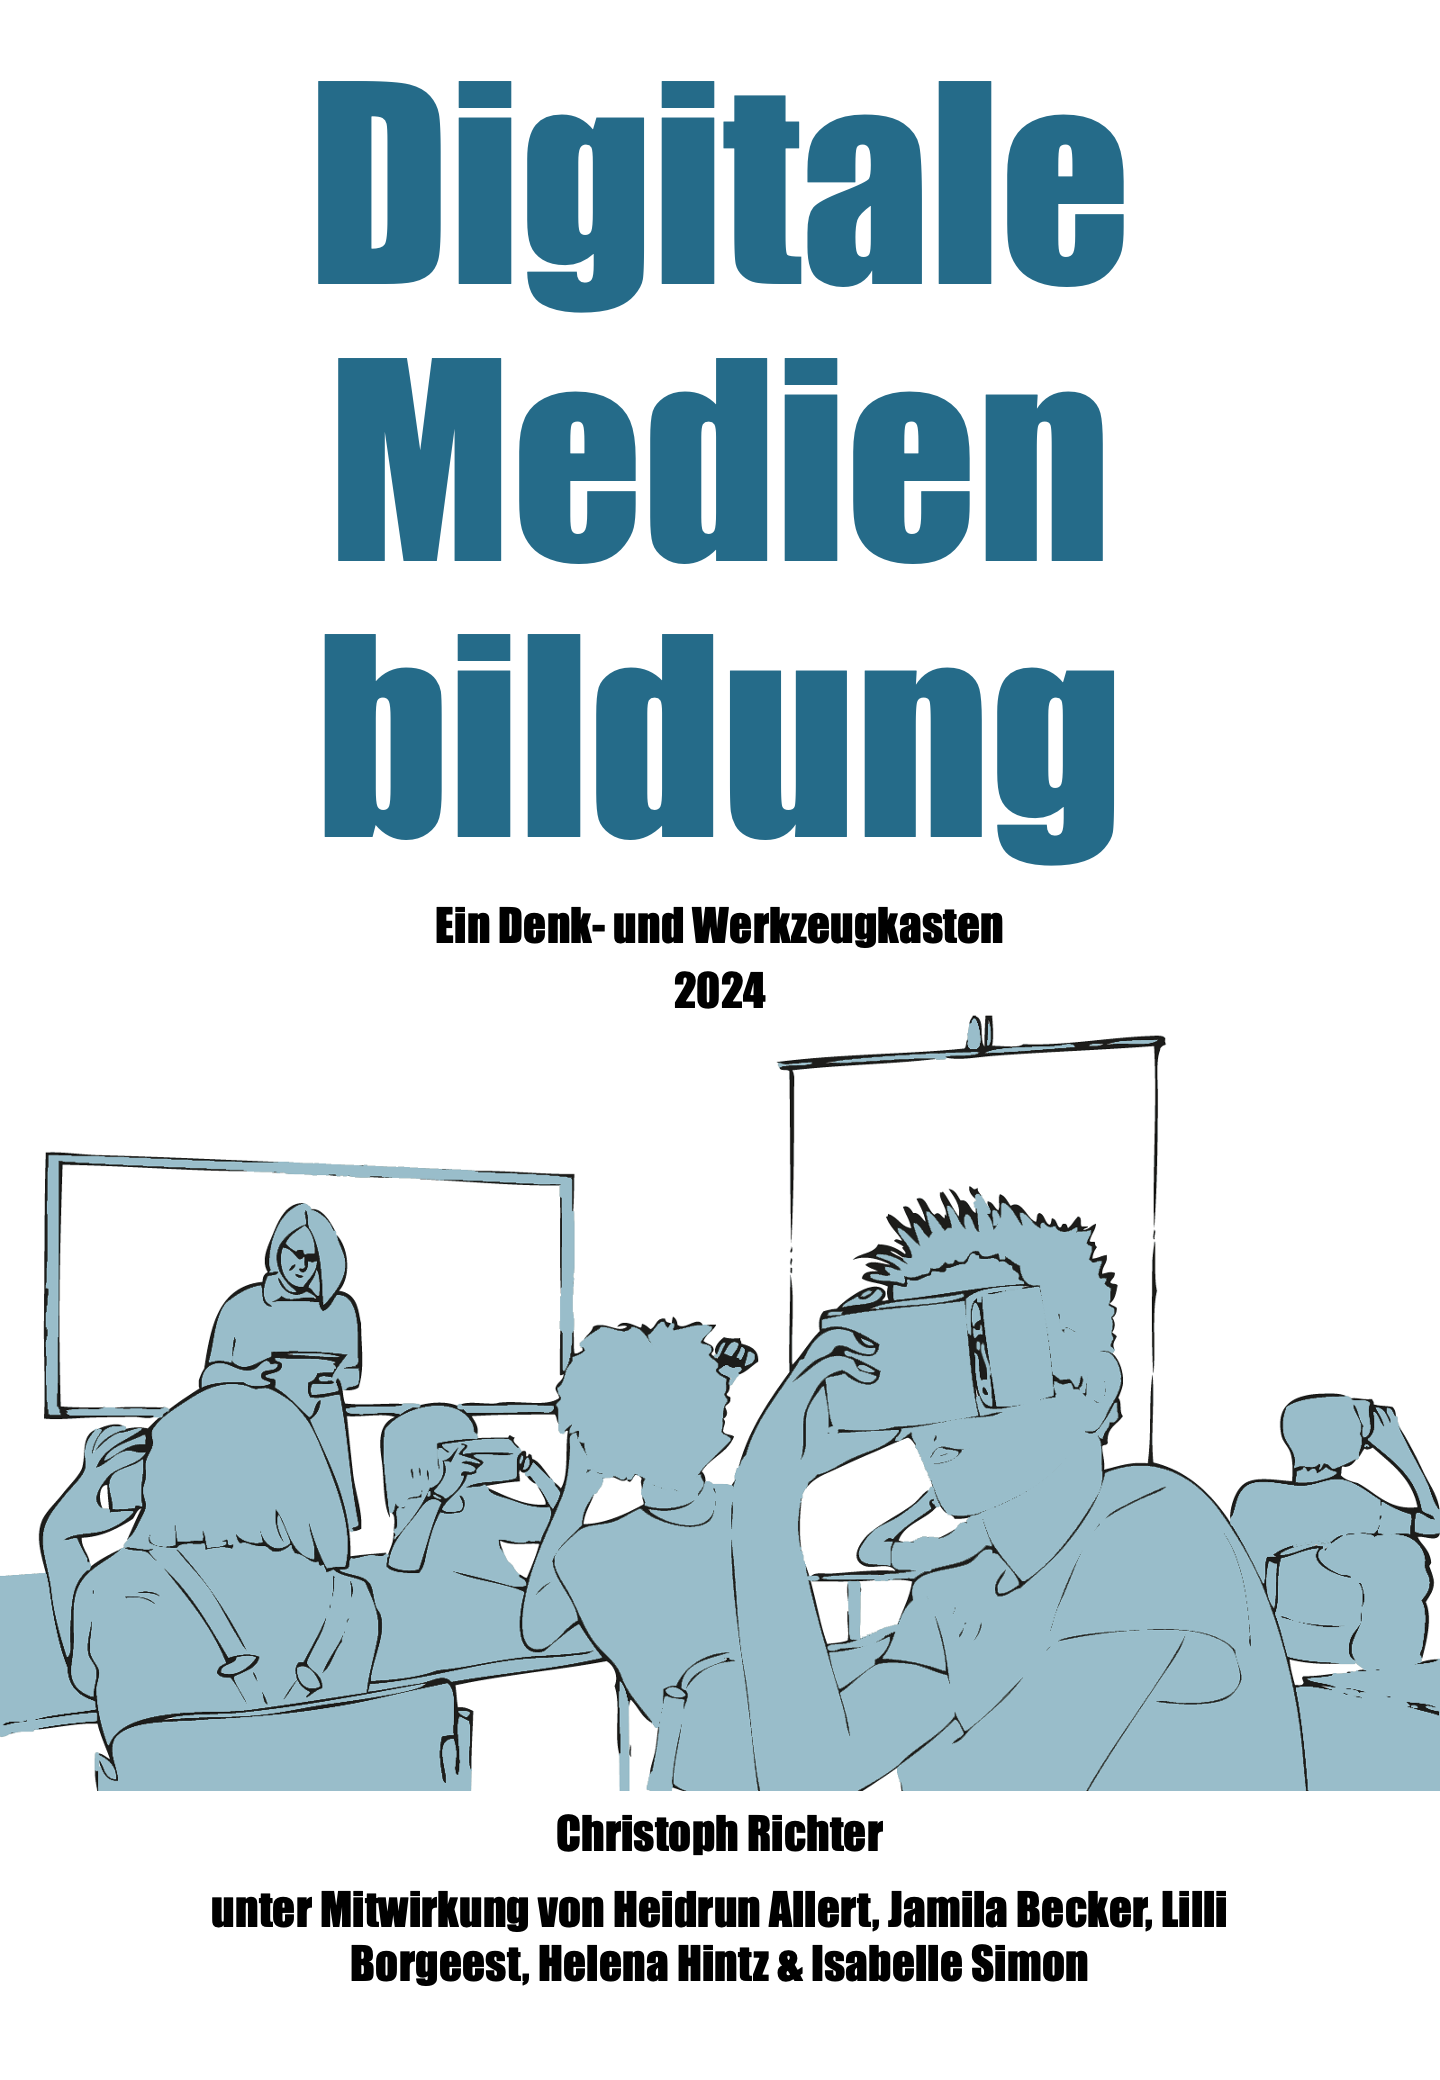
\includegraphics[width=\textwidth, height=0.99\textheight]{Figures/Cover.png}


\newpage
~\vfill
\thispagestyle{empty}

\noindent IMPRESSUM\\
\noindent »Digitale Medienbildung - Ein Denk- und Werkzeugkasten«\\
\noindent Christoph Richter\\
\noindent unter Mitwirkung von Heidrun Allert, Jamila Becker, Lilli Borgeest, Helena Hintz und Isabelle Simon\\
\\
\noindent 2024\\
\\
\noindent Herausgeberin:\\
Heidrun Allert\\
Olshausenstr. 75\\
24118 Kiel\\
Deutschland\\
allert(at)paedagogik.uni-kiel.de\\
\\
\noindent Web: \href{https://christoph-mp.github.io/Digitale-Medienbildung/}{christoph-mp.github.io/Digitale-Medienbildung}\\ % URL

\noindent DOI: \href{https://zenodo.org/records/13778113}{10.5281/zenodo.13778113}\\ % DOI


\includegraphics[width=0.15\textwidth]{"Figures/by-sa.png"}\par\vspace{1cm}


\noindent Dieses Werk ist unter der Creative-Commons-Lizenz Namensnennung – Weitergabe unter gleichen Bedingungen 4.0 International \href{https://creativecommons.org/licenses/by-sa/4.0/}{CC BY-SA 4.0} Lizenz veröffentlicht. Den vollständigen Lizenztext finden Sie unter \href{https://creativecommons.org/licenses/by-sa/4.0/deed.de}{https://creativecommons.org/licenses/by-sa/4.0/deed.de}.\\ % License information


\newpage
\pagenumbering{arabic}
